\documentclass[preprintnumbers,amsmath,amssymb,onecolumn,12pt]{revtex4-2}
\usepackage{graphicx}% Include figure files
\usepackage{dcolumn}% Align table columns on decimal point
\usepackage{bm}% bold math
\usepackage{natbib}
\usepackage{physics}
\usepackage[caption=false]{subfig}
\newcommand{\be}{\begin{equation}}
\newcommand{\ee}{\end{equation}}

\newcommand{\bea}{\begin{eqnarray}}
\newcommand{\eea}{\end{eqnarray}}
 
\def\sgn{\mathop{\rm sgn}}

\begin{document}
\vspace{0.2in}
{\Large \hspace{1.6in}\textsc{Supplementary Material} }\\
\
\title{Low field depolarization of electronic spins through dipole-dipole coupling}

\author{C. Pellet-Mary$^1$, M. Perdriat$^1$, G. H\'etet$^1$} 

\affiliation{Laboratoire De Physique de l'\'Ecole Normale Sup\'erieure, \'Ecole Normale Sup\'erieure, PSL Research University, CNRS, Sorbonne Universit\'e, Universit\'e Paris Cit\'e , 24 rue Lhomond, 75231 Paris Cedex 05, France.}

\maketitle

\tableofcontents

\section{NV$^-$ ground state Hamiltonian in low magnetic field}
\begin{figure}
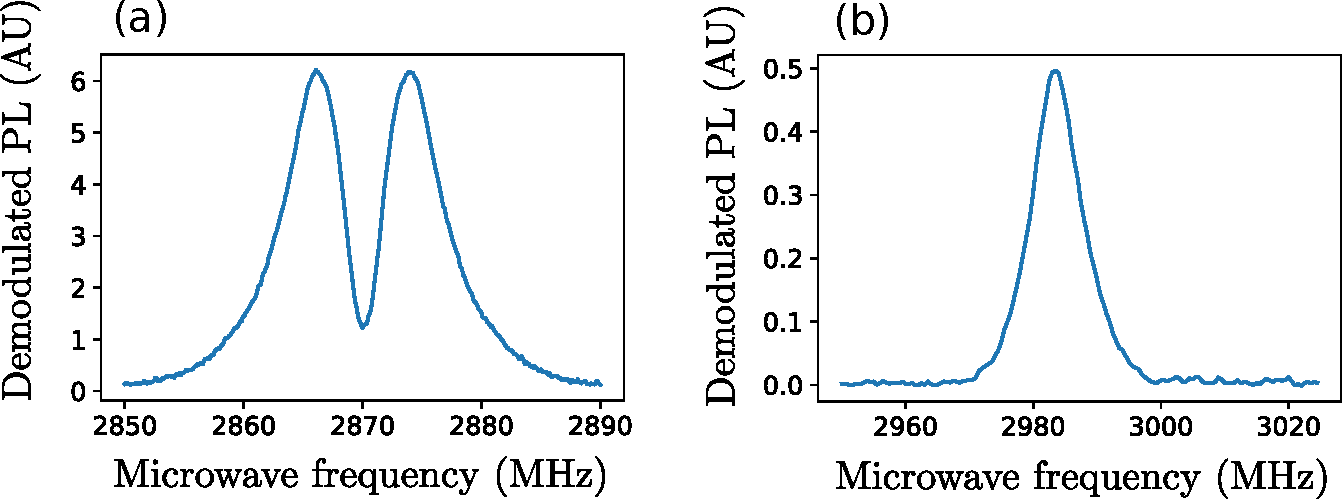
\includegraphics[width=0.9\textwidth]{Figures_SI/fig_ESR}
\caption{ODMR measurement (a) in zero magnetic field, (b) in non-zero magnetic field when zooming on a single class transition}
\label{ESR_single_spin}
\end{figure}
With zero external magnetic field, there are three possible sources of splitting of the $\{\ket{+1},\ket{-1}\}$ manifold : local electric field, crystal strain and local magnetic field.Of these three causes, only the electric field can explain the shape of the ODMR line that we observe in zero external magnetic field (Fig. \ref{ESR_single_spin}a) \cite{mittiga2018imaging}.

Indeed, a random local magnetic field would produce a single broadened line, and the crystal strain would produce a shifting of the zero field splitting (ZFS) comparable its splitting, which would also blur the two transitions into a single line. On the other hand, due to the large difference between the longitudinal and transverse electric field susceptibilities ($d_\parallel = 0.35\ \rm Hz\, cm/V$ and $d_\perp = 17\ \rm Hz\, cm/V$ \cite{van1990electric}), random local electric field will, on average, cause a splitting much stronger than its ZFS shifting and result in a two peak spectrum.

We will therefore neglect the contribution of the strain, local magnetic field and longitudinal electric field,  as well as the hyper-fine structure of the NV center because of the large inhomogeneous broadening of the transitions (Fig. \ref{ESR_single_spin}b) and we will consider the following spin Hamiltonian for the NV$^-$ ground state :
\begin{equation}
\mathcal{H}_s=D S_z^2 + \gamma_e \vec{B}_{\rm ext} \cdot \vec{S}+ d_\perp \left[ E_x(S_y^2-S_x^2) + E_y(S_xS_y+S_yS_x) \right]
\end{equation}
Where $D=2.87\ \rm GHz$ is the zero field splitting and $\gamma_e=2.8\ \rm MHz/G$ the gyromagnetic ratio of the electron.

In the absence of an external magnetic field, the symmetry in the ($xy$) plane allows us to chose the $x$ direction along the electric field, therefore the eigenstates of $\mathcal{H}_s$ become $\{ \ket{0},\ket{+}=\frac{\ket{+1}+\ket{-1}}{\sqrt{2}},\ket{-}=\frac{\ket{+1}-\ket{-1}}{\sqrt{2}} \} $.

In the presence of non-zero magnetic field, let us call the Hamiltonian eigenstates $\{ \ket{g},\ket{d}, \ket{e} \} $. Fig. \ref{map etats propres} shows how close the $\ket{e}$ state is to the $\ket{+1}$ and $\ket{+}$ states as a function of the external magnetic field. Looking at the closeness of $\ket{d}$ to $\ket{-1}$ and $\ket{-}$ would show similar results, while $\ket{g}$ is pretty much equals to $\ket{0}$ for $B<100\ \rm G$.

This tells us that in most cases, the $\{ \ket{0},\ket{+},\ket{-} \}$ basis is only the good Hamiltonian basis for magnetic field smaller than a few Gauss, except in the case of pure transverse magnetic field where the $\{ \ket{0},\ket{+},\ket{-} \}$ basis remains a good basis even for sizable magnetic fields.
\begin{figure}
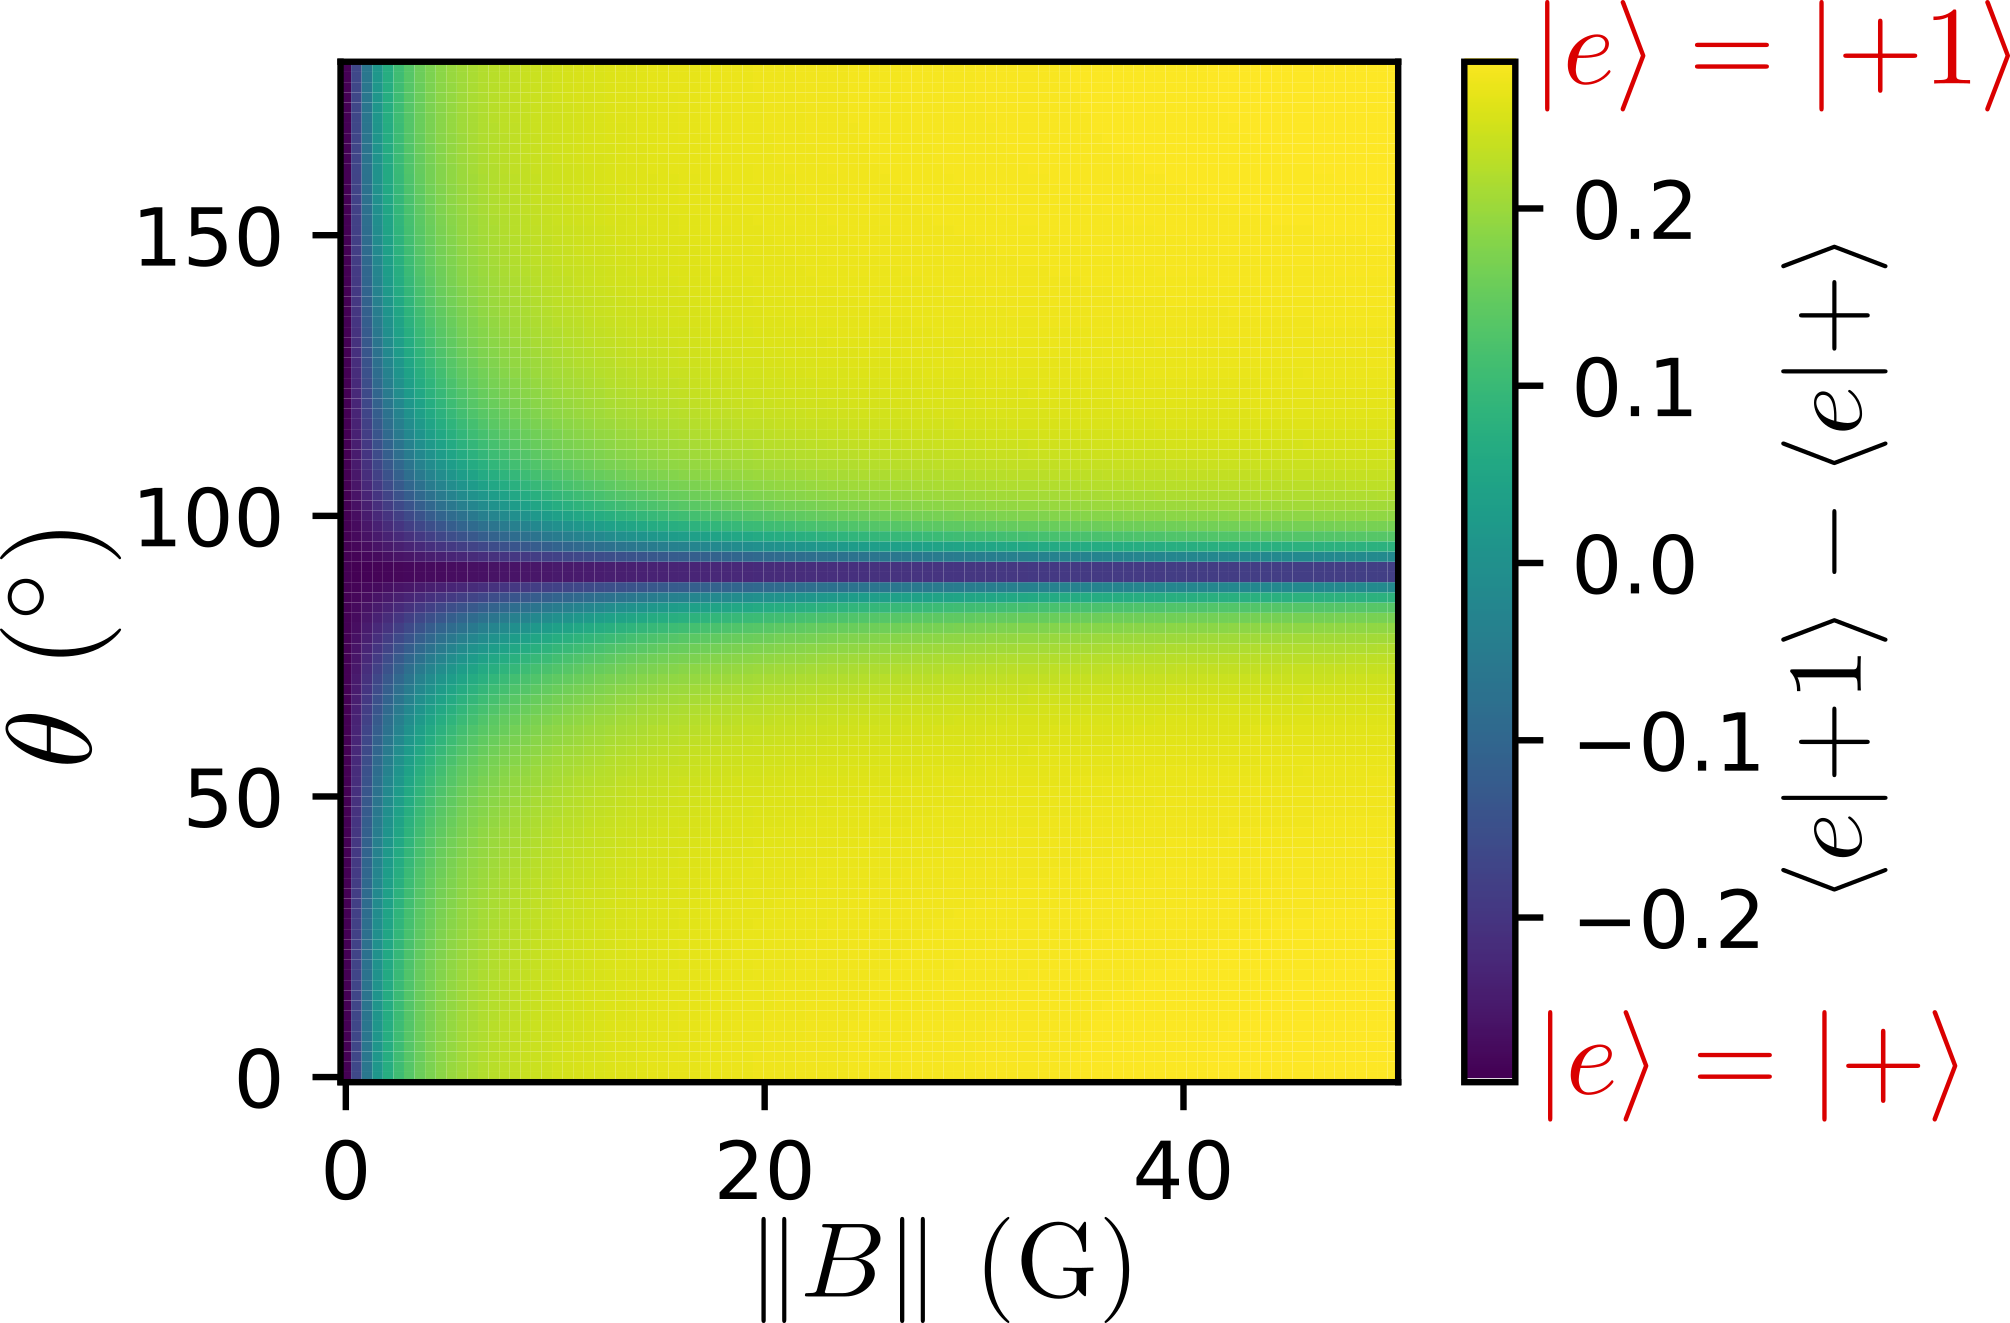
\includegraphics[width=0.7\textwidth]{Figures_SI/map_etats_propres}
\caption{Closeness of the Hamiltonian most excited state $\ket{e}$ with the states $\ket{+1}$ and $\ket{+}$ as a function of the magnetic field amplitude and angle $\theta$ with respect to the NV axis.}
\label{map etats propres}
\end{figure}


\section{Samples}
A faire à la fin pour être sur des figures du main text.
\section{Experimental Setup}
\begin{figure}
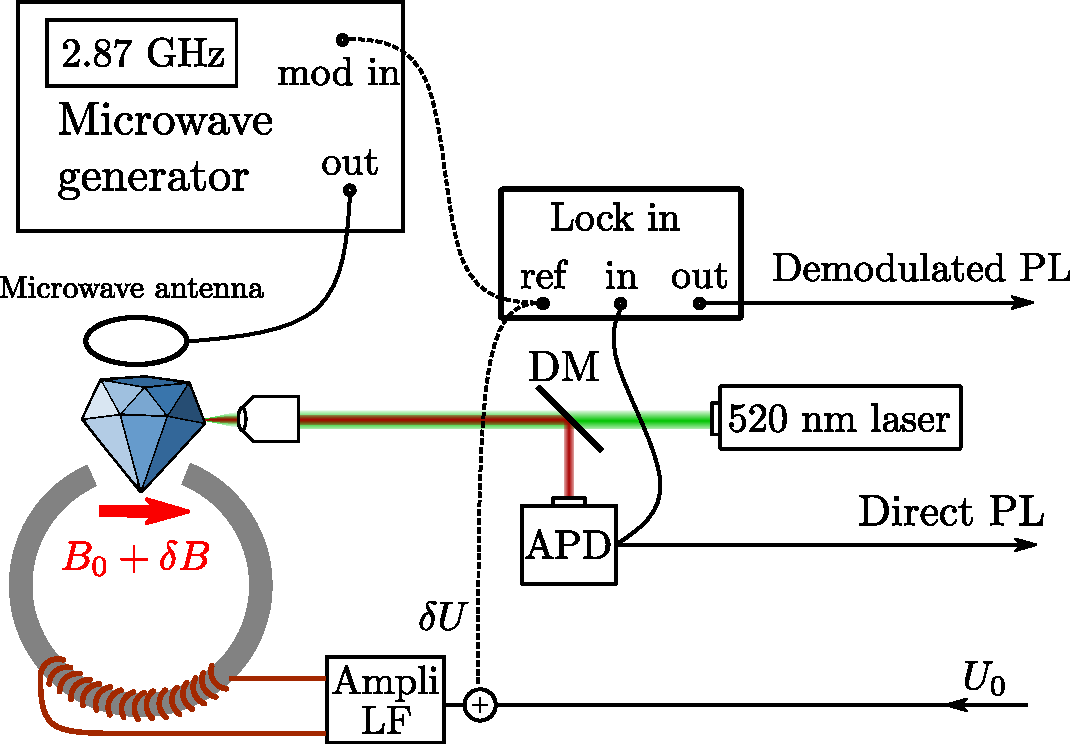
\includegraphics[width=0.7\textwidth]{Figures_SI/shema_exp}
\caption{Experimental Setup}
\label{setup}
\end{figure}
Fig. \ref{setup} shows the general purpose experimental setup used for all the experiments presented in this article.

The optical polarization and readout of the spins is done by focusing a green laser on the diamond sample with an objective lens([ref]), and collecting the back-scattered red fluorescence from the NV center on an avalanche photo-diode (APD, REF). The laser is filtered out using a dichroic mirror (DM, ref) and a notch filter. The NV$^0$ fluorescence is filtered using an additional 645 nm longpass filter.

The laser used here is a [REF], providing pulses of X ns at a rate of 20 MHz, with an average power of $0.5 \sim 5\ \rm mW$. The trigger of the pulses is generated externally in order to achieve fast  gating of the laser for the $T_1$ measurement. We previously did similar experiment using a continuous 532 nm laser and observed no difference in the behavior of the spins.

The magnetic field is provided by a homemade electromagnet composed of a c-shape iron core and  copper wires. The magnet is mounted on two mechanical rotation stages, allowing a control on the polar and azimuthal angle of the magnetic field within a fraction of a degree and is alimented through a low frequency amplifier (REF)

The microwave field is generated by a Rhode \& Shwarz SMB 100A and is emitted with a handmade loop antenna. The field is gated by a [REF minicircuit] switch controlled externally.

A lock-in amplifier is used either to modulate the microwave amplitude for ODMR measurement, or to add an oscillatory magnetic field for the magnetometry protocol. In both case we use a modulation frequency $\sim 1\ \rm kHz$ and demodulate the APD signal.
\section{Experimental details}
\subsection{$T_1$ fitting Protocol}
The $T_1$ profile that we observe with our samples is neither purely exponential, nor purely stretched exponential, which is to be expected when the dipole-dipole spin decay is comparable to the phonon decay.

Fig. \ref{T1_fits} shows the result of a lifetime measurement, measured with the subtraction protocol described in the main text, for zero and non-zero magnetic field. The result is fitted with exponential and stretched-exponential (with a stretch factor $\beta=0.5$) functions. We can see that for the shorter lifetime (0B), the measurement follows more closely the stretched-exponential profile, while the longer lifetime is closer to the exponential one (except at very short times).

In order to directly compare the results from different magnetic fields, we therefore decided to fit each $T_1$ measurement with both a stretched and exponential decay : $S(\tau)=A \exp (-\frac{\tau}{T_1^{\rm ph}} -\sqrt{\frac{\tau}{T_1^{\rm dd}}})$.
In order to add consistency to the measurement of $T_1^{\rm dd}$, we decided to fix $T_1^{\rm ph}$ for each sample, leaving $T_1^{\rm dd}$ as the only free parameter in the fitting procedure. The value chosen for samples [REF] and [REF] was $T_1^{\rm ph}=3.62\ \rm ms$. Fig. 1 of the main text shows the result of fitting the same two measurement with this formula.

An other possibility would be to use an arbitrary stretched factor in the fitting function : $S(\tau)=A \exp (-(\frac{\tau}{T_1^{\rm ph}})^\beta )$. Fig. \ref{alphas} shows the optimal $\beta$ parameter as a function of the external magnetic field, which confirms that the $T_1$ profile gets closer to a pure stretched-exponential in zero magnetic field.
\begin{figure}
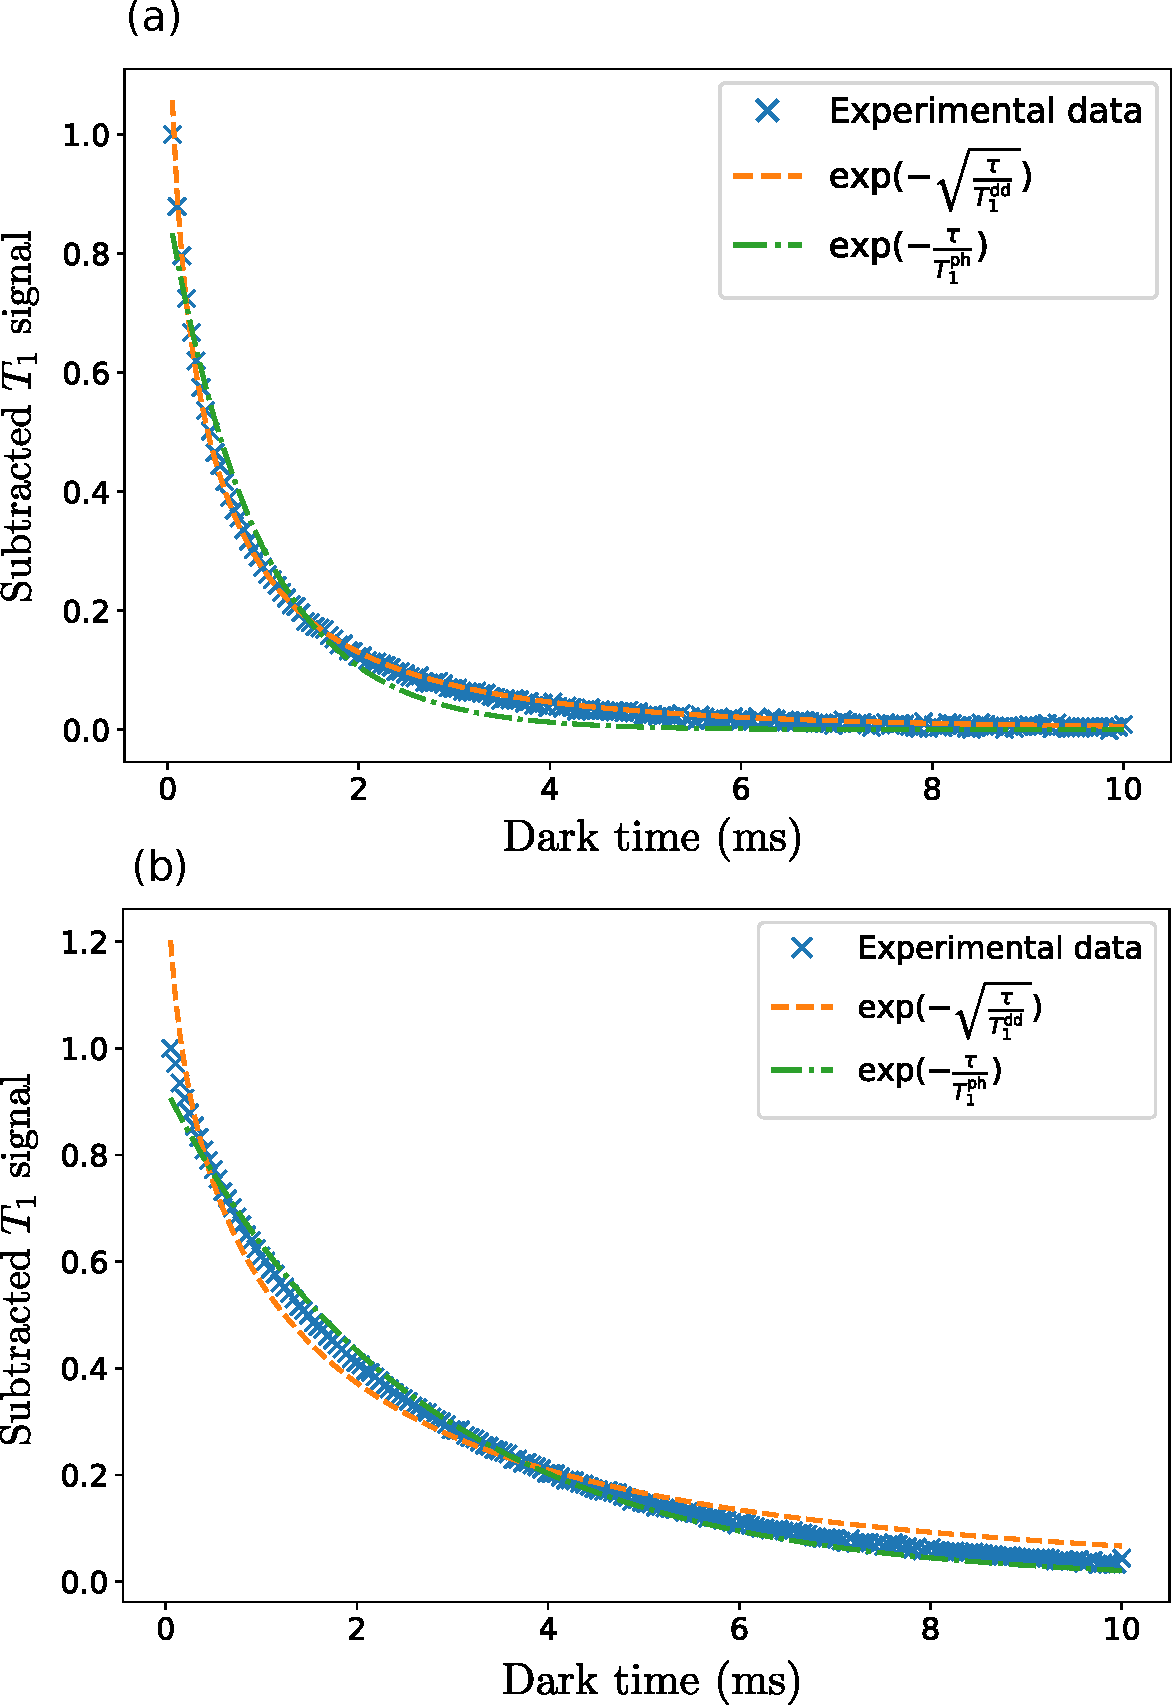
\includegraphics[width=0.8\textwidth]{Figures_SI/Fig_T1_combined}
\caption{$T_1$ measurement with purely exponential and purely stretched exponential fits (a) in zero magnetic field (b) in non-zero magnetic field}
\label{T1_fits}
\end{figure}
\begin{figure}
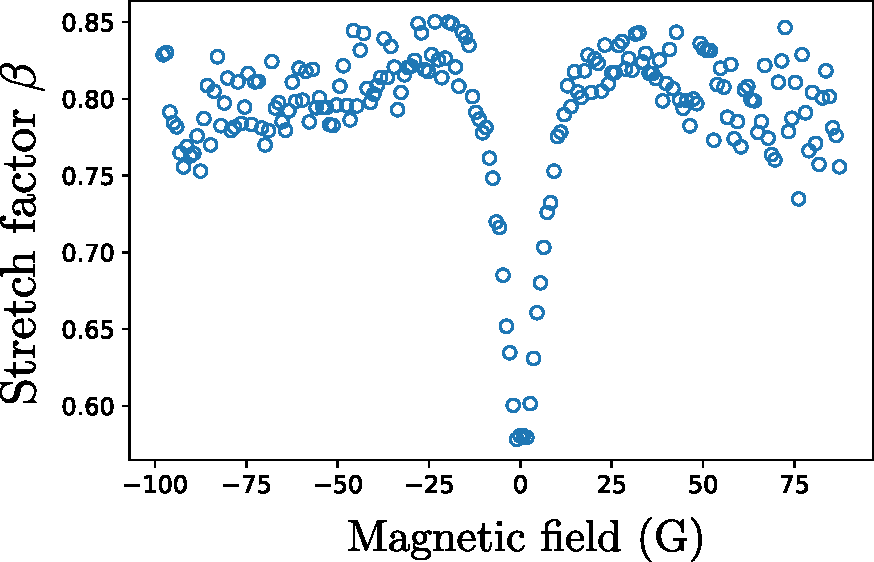
\includegraphics[width=0.45\textwidth]{Figures_SI/fig_alphas}
\caption{Best stretch factor $\beta$ for a $T_1$ fit of the form $f(\tau)=A \exp(-(\frac{\tau}{T_1})^\beta)$ as a function of a randomly oriented magnetic field amplitude}
\label{alphas}
\end{figure}
\subsection{Spectral range of the dipole-dipole cross-relaxations}
\begin{figure}
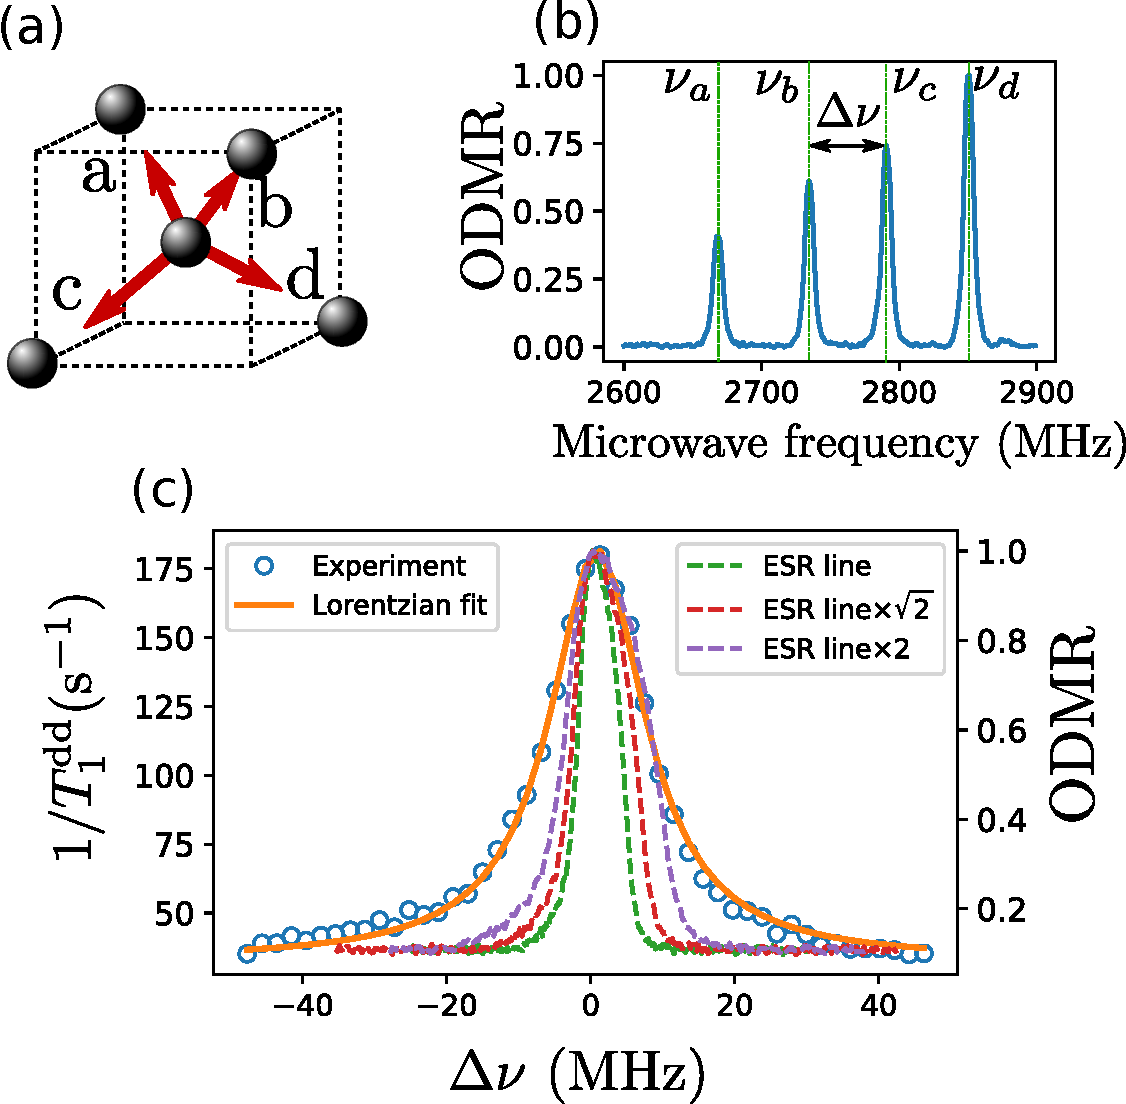
\includegraphics[width=0.7\textwidth]{Figures_SI/largeur_fluct_SI}
\caption{Dipole-dipole depolarization for two near-resonant classes. (a) Sketch of the four possible orientations ("classes") in a single crystal diamond lattice. (b) ODMR spectrum showing four $\ket{0} \to \ket{-1}$ resonances corresponding to the four spin classes. The detuning $\Delta \nu$ between the classes b and c was controlled by changing the orientation of the external magnetic field.(c) Stretch part of the lifetime decay for the spins resonant with $\nu_c$ as a function of the detuning $\Delta \nu$ (blue circles), fitted by a Lorentzian with half width at half maximum 8.04 MHz. Single class ESR line stretched by a factor of 1,$\sqrt{2}$ and 2 are added for comparison}
\label{largeur_fluct}
\end{figure}
In the absence of other 

An experimental signature of the fluctuator hypothesis developed in \cite{choi_depolarization_2017} is to measure the depolarization rate for two near-resonant classes : if there are indeed very fast decaying NV centers (fluctuators with lifetime $T_1^f < 100 ns$), then the spectral width of the fluctuator would be increased beyond $1/T_2^*$ (which we assume to be homogeneous among all spins in the crystal), which means that they would be able to exchange spin quanta (flip-flop) with non-resonant NV detuned by $\Delta \nu$ such that $2\pi/T_1^f > \Delta \nu > 2\pi/T_2^*$

In order to verify this claim, we have to measure the spectral overlap between two classes, which in the absence of fluctuator should be proportional to the flip-flop rate, and compare it to the actual flip-flop rate which we can measure through the depolarization rate of the spins.

Fig. \ref{largeur_fluct} shows the results of such an experiment where we measured the stretched part of the NV's decay rate, which is very well fitted by a Lorentzian of width $\sigma=8.04 MHz$, and compare it to an ODMR line of a single class of NV centers, stretched by a factor of $\sqrt{2}$ and 2 to simulate the spectral overlap of the two classes (discussed bellow). One should notice that, not only is $1/T_1^{\rm dd}$ significantly larger than the ODMR profile, it also doesn't have the same shape. 

We should not that this broadening can not be explained by the dipole-dipole interaction strength : for a sample with 3 ppm of NV centers, the average dipole-dipole interaction strength between two nearest NV centers $J_0/r^3 \sim 27\ \rm kHz$ which is several order of magnitude lower than the broadening we observe. 

\begin{figure}
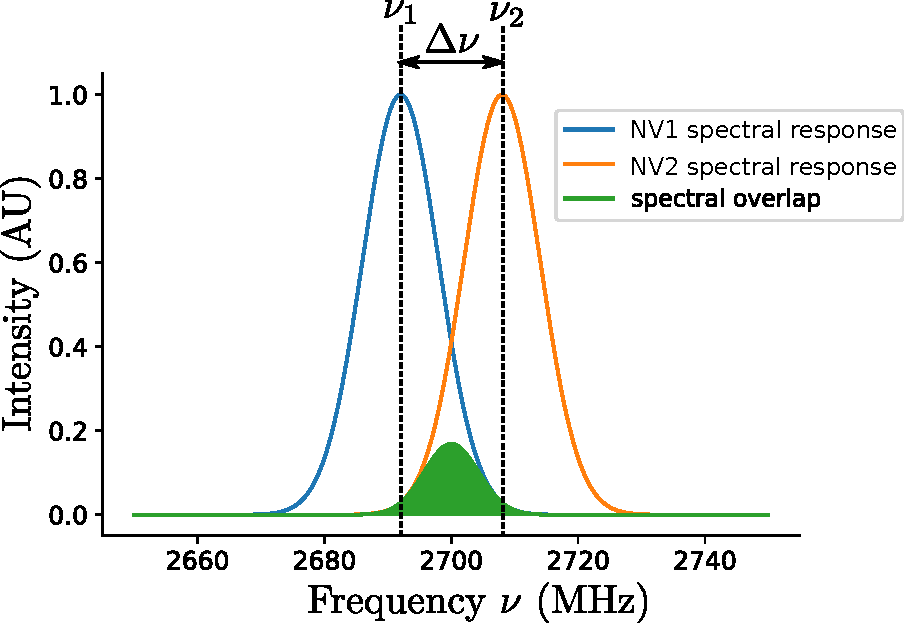
\includegraphics[width=0.7\textwidth]{Figures_SI/overlap}
\caption{Illustration of the spectral overlap for two gaussian spectra}
\label{overlap}
\end{figure}

As illustrated on Fig. \ref{overlap}, we define the spectral overlap $S(\Delta \nu)$ between two spins of spectral response $S_1(\nu)$ and $S_2(\nu)$, centered respectively on the frequencies $\nu_1$ and $\nu_2$ where $\Delta \nu = \nu_2-\nu_1$ as :
\begin{equation}
S(\Delta \nu)=\int S_1(\nu, \nu_1)S_2(\nu, \nu_2) d\nu
\end{equation}
In order to approximate the spectral overlap in our experiment, we will consider the analytical solution in the Gaussian and Lorentzian case :

\begin{itemize}
\item For two gaussians of standard deviation $\sigma$, the spectral overlap as a function of the detuning $\Delta \nu = \nu_1-\nu_2$ is itself a gaussian of standard deviation $\sigma'=\sqrt{2} \sigma$. :
\begin{align*}
S(\Delta \nu)&\propto \int \exp(-\frac{(\nu-\nu_1)^2}{2\sigma^2})\exp(-\frac{(\nu-\nu_2)^2}{2\sigma^2}) d\nu \\
&\propto\exp(-\frac{(\Delta \nu)^2}{4\sigma^2})
\end{align*}

\item For two Lorentzian profile with width $\sigma$, the overlap function is itself a Lorentizan with width $\sigma'=2\sigma$ :
\begin{align*}
S(\Delta \nu)&\propto \int \frac{1}{1+ \frac{(\nu-\nu_1)^2}{\sigma^2}}\cdot \frac{1}{1+ \frac{(\nu-\nu_2)^2}{\sigma^2}} d\nu \\
&\propto\frac{1}{1+ \frac{(\Delta \nu)^2}{4\sigma^2}}
\end{align*}
\end{itemize}

The ODMR lines that we measure are neither Lorentzian nor Gaussian (although they tend to be closer to Gaussians), and can even be asymmetric. Nevertheless, the overlap between two classes can most likely be approximated by a single class ODMR profile stretched by a factor between $\sqrt{2}$ and 2.


\section{Les détails qui tuent}
\subsection{Effect of laser polarization}
\begin{figure}
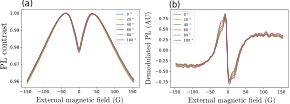
\includegraphics[width=0.9\textwidth]{Figures_SI/fig_Pola}
\caption{Effect of the polarization of the incident laser. (a) Photoluminescence as a function of randomly oriented magnetic field amplitude for various polarization angle. (b) Demodulated PL in the same conditions}
\label{Pola}
\end{figure}
\subsection{Alignment of B}
La faudrait p-e montrer ce qu'il se passe pour un décalage de quelques degrés. A voir si j'ai déja les plots
\section{Fluctuator et tout}
\subsection{121 VS 22}
\subsection{100 vs 0B}

\bibliographystyle{plain}
\bibliography{CR_SI}{}
\end{document}